\documentclass[11pt,a4paper]{report}
\usepackage{geometry}
\usepackage{latexsym}
\usepackage{graphicx}
\usepackage{amsmath}
\usepackage[spanish]{babel}
\usepackage{multirow}
\usepackage{amssymb}
\usepackage{tikz}
\usepackage{subcaption}
\usepackage{natbib}

\newcommand*\circled[1]{\tikz[baseline=(char.base)]{
		\node[shape=circle,draw,inner sep=2pt] (char) {#1};}}
	

\setlength{\parindent}{0pt}

\date{}
\begin{document}
\title{Memoria Trabajo Lingüística Computacional}
\author{  Miguel This is a Placeholder\and Roberto Labadie Tamayo}
	\date{Octubre 2022}
	\maketitle
	
	
	\section*{Tarea I}
		
		Para evaluar la tarea de etiquetado morfosintágtico empleando un HMM entrenado sobre el corpus \textbf{cess-esp} se estudian dos variantes, una sobre una versión reducida del problema con un conjunto de categorías mas abarcadoras y la versión original usando las etiquetas tal cual aparecen en el corpus.
		\\
		A través de una validación cruzada con 10 particiones del dataset se obtienen los resultados como se muestran en la \figurename~\ref{HMM_task1}.
		
		\begin{figure}[!thb]
		\begin{center}
			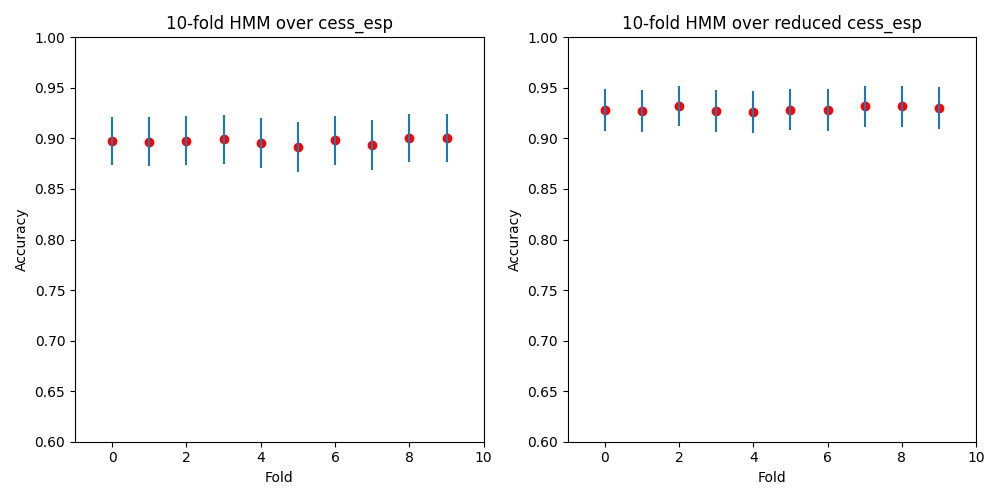
\includegraphics[scale=0.6]{images/HMM_task1.png}
		\end{center}
		\caption{Hidden Markov Model sobre cess-esp (izquierda) y cess-esp reducido (derecha) }
		\label{HMM_task1}
	\end{figure}
	
	Como se puede apreciar el desempeño del modelo es mejor para el dataset de la tarea reducida gracias a que la cantidad de estados ocultos del modelo es menor por tanto la posibilidad de escoger una transición errada disminuye, esta observación se puede realizar incluyendo además los intervalos de un  un 95\% de confianza. Nótese ademas que en ambos modelos la $i-esima$ partición es exactamente la misma, i.e., el mismo conjunto de elementos ordenados en ambos modelos. En el \tablename~\ref{HMM_task1_table} se muestran de manera detallada los resultados para cada variante.
		\begin{table}[thb!]
		\begin{center} 		
			\begin{tabular}{cc} 
				\hline	
				\multirow{2}{*}{\textbf{cess-esp}}&\textbf{reduced}\\
				&\textbf{cess-esp}\\
				\hline
				0.897$\pm$0.02&0.928$\pm$0.02\\
				0.897$\pm$0.02&0.927$\pm$0.02\\
				0.898$\pm$0.02&0.932$\pm$0.02\\
				0.899$\pm$0.02&0.928$\pm$0.02\\
				0.896$\pm$0.02&0.927$\pm$0.02\\
				0.892$\pm$0.02&0.928$\pm$0.02\\
				0.898$\pm$0.02&0.928$\pm$0.02\\
				0.893$\pm$0.02&0.932$\pm$0.02\\
				0.900$\pm$0.02&0.932$\pm$0.02\\
				0.900$\pm$0.02&0.930$\pm$0.02\\
				\hline
			\end{tabular}
			\caption{Perplejidad sobre modelos de 3-gramas y 4-gramas}	
			\label{HMM_task1_table}
		\end{center}
	\end{table}		 	
	\\\\\\\\\\\\\\\\

	
	Teniendo en cuenta que la medida de accuracy nos da un valor suavizado del desempeño global de todas las etiquetas, analizamos la media de Macro-F1 para cada partición como se muestra en la \figurename~\ref{macro-f1-hmm}.
	
	\begin{figure}[!thb]
		\begin{center}
			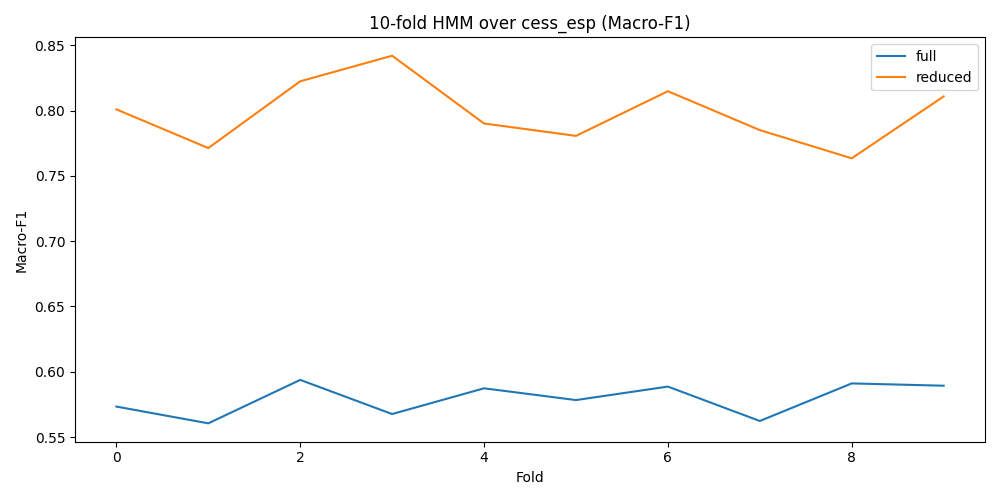
\includegraphics[scale=0.6]{images/macro-f1-hmm.png}
		\end{center}
		\caption{Macro-F1 Hidden Markov Model sobre cess-esp y cess-esp reducido}
		\label{macro-f1-hmm}
	\end{figure}

	De aquí podemos concluir que evidentemente hay etiquetas que están siendo muy mal predichas por el modelo, sobretodo para la tarea ampliada, lo que puede estar relacionado con una subrepresentación de estos fenómenos en el training-set. Teniendo en cuenta esto, resulta más coherente asumir un etiquetado más global y suavizado que permita tener para cada categoría más ejemplos de entrenamiento como el propuesto en la tarea reducida. En lo adelante emplearemos el conjunto de datos reducidos para evaluar los modelos.
	
	\section*{Tarea II}
	
	Luego de barajar el dataset para la tarea reducida y tomar los últimos $\Big\lceil \frac{|\mathcal{D}|}{10}\Big\rceil$ elementos para validar nuestro modelo, se observa una relación directamente proporcional con el acuraccy y la cantidad de datos empleados para entrenamiento como se muestra en la \figurename~\ref{incremental-set}.
		
		
		\begin{figure}[!thb]
			\begin{center}
				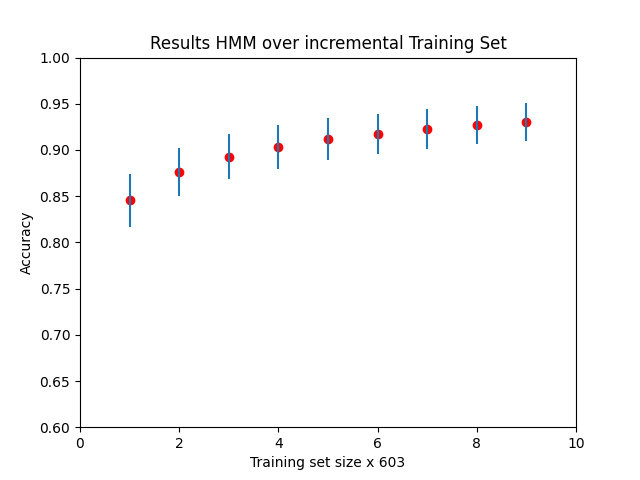
\includegraphics[scale=0.6]{images/incremental-set.png}
			\end{center}
			\caption{ Accuracy Hidden Markov Model sobre cess-esp reducido y con incremento progresivo del conjunto de entrenamiento}
			\label{incremental-set}
		\end{figure}
	Efectivamente alcanzando el mejor desempeño para el conjunto de entrenamiento completo. Al igual que en la tarea anterior cuando empleamos el dataset ampliado y algunas etiquetas resultaban subrepresentadas, es posible concluir que en este caso sucede lo mismo para subconjuntos pequeños del dataset. Por otro lado dentro de un modelo estadístico como lo es el HMM, el número de observaciones de un suceso esta directamente relacionado con cuan preciso es el valor de probabilidad de ocurrencia calculado para este.
	
	\section*{Tarea III}
	
	Para incorporar al Tnt el método de suavizado para palabras desconocidas mediante el uso de sufijos, primero estudiamos el comportamiento del método Affix Tagger  con varias longitudes de sufijos en el rango de 1 a 9 caracteres, en la ~\figurename~\ref{affix} se muestra el valor medio del accuracy para este método en un cross-validation que involucra el mismo conjunto de datos ordenados en cada fold para cada variante de sufijo.
	
	\begin{figure}[!thb]
		\begin{center}
			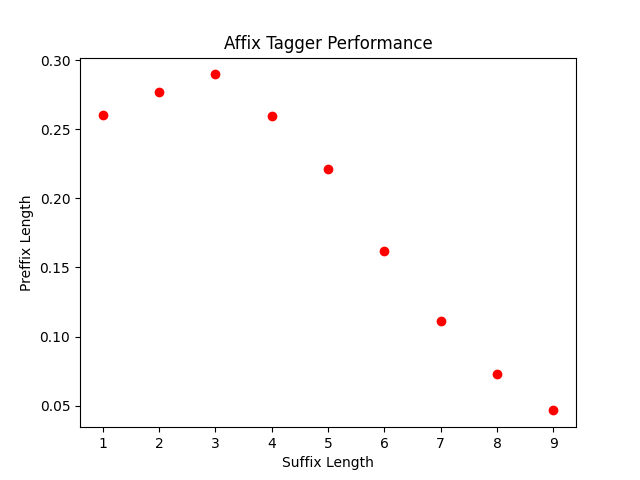
\includegraphics[scale=0.6]{images/affix.png}
		\end{center}
		\caption{ Accuracy Medio del método Affix Tagger sobre cross-validation en cess-esp reducido.}
		\label{affix}
	\end{figure}

	del anterior experimento, tomamos como longitud de sufijos para estudiar el suavizado en el Tnt $l=3$.


\end{document}